\documentclass[crop,tikz]{standalone}

\usepackage{amsmath}
\tikzset{>=latex}

\begin{document}
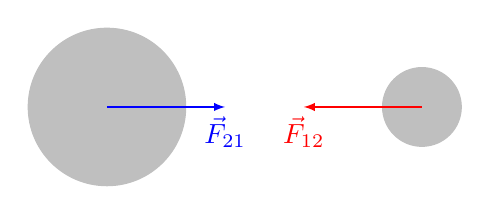
\begin{tikzpicture}
  \draw[gray!50,fill] (-2,0) circle (1)   coordinate (c1);
  \draw[gray!50,fill] (+2,0) circle (0.5) coordinate (c2);
  \draw[->,blue] (c1) -- ++(+1.5,0) node[below] {$\vec{F}_{21}$};
  \draw[->,red]  (c2) -- ++(-1.5,0) node[below] {$\vec{F}_{12}$};
\end{tikzpicture}
\end{document}
